\documentclass{beamer}

\usepackage{default}
\usepackage{color}
\usepackage{graphicx}
\usepackage{animate}
\usepackage{hyperref}
\setbeamertemplate{navigation symbols}{}%remove navigation symbols
\begin{document}
\title{Where am I? The symmedian point!}   
\author{Bill Lionheart} 

\frame{\titlepage}




\begin{frame} \frametitle{What if the GPS goes off?}
\begin{center}
If the satellite navigation system (GPS,GLONASS) fails how can ships find their position?
\end{center}
\pause
\begin{center}
Use the old fashioned method of {\color{red}Celestial Navigation.} \\
Measuring the position of the stars and planets and an accurate clock to find our position.
\end{center}

\end{frame}

\begin{frame} \frametitle{How to do it}
\begin{enumerate}
\item<1-> Identify the stars or planets you can use.
\item<2-> Measure the angle it makes to horizon $H_o$ and note time. 
\item<3-> Look up the point on the earth where that object is directly overhead (GP)
\item<4-> From an {\em assumed position} AP work out the angle it should make to the horizon and its compass direction (azimuth).
\item<5-> Difference between measured $H_o$ and calculated $H_c$ angle and the bearing gives you a position line (LOP). 
\end{enumerate}
\vspace{-0.6cm}
\includegraphics[scale=0.19,angle=-90,origin=c]{HoHc.pdf}
%\includegraphics[scale=0.5]{intercept1-300x300}

%{\tiny Diagram from blueplanetcruisingschool.com}

\end{frame}


\begin{frame}\frametitle{Sextant animation}

%\url{https://en.wikipedia.org/wiki/Sextant#/media/File:Using_sextant_swing.gif}

\only<1>{\includegraphics[width=\linewidth]{sextant-0}}

\only<2>{\includegraphics[width=\linewidth]{sextant-1}}
\only<3>{\includegraphics[width=\linewidth]{sextant-5}}
\only<4>{\includegraphics[width=\linewidth]{sextant-10}}
\only<5>{\includegraphics[width=\linewidth]{sextant-15}}
\only<6>{\includegraphics[width=\linewidth]{sextant-16}}
\only<7>{\includegraphics[width=\linewidth]{sextant-18}}
\only<8>{\includegraphics[width=\linewidth]{sextant-20}}
\only<9>{\includegraphics[width=\linewidth]{sextant-25}}
\only<10>{\includegraphics[width=\linewidth]{sextant-26}}

\only<10-> {\tiny Animation from Wikipedia/Sextant(Marine) Joaquim Alves Gaspar CC BY-SA 2.5}


%  \animategraphics[loop,controls,width=\linewidth]{12}{sextant-}{0}{27}

\end{frame}

\begin{frame}\frametitle{Three lines don't meet at a point!}

\includegraphics[width=\linewidth]{threelines.eps}

\end{frame}

\begin{frame}\frametitle{Solve three equations in two variables}
\only<1->{$$
\begin{array}{c}
 a_{11} x_1+a_{12} x_2 =b_1\\
 a_{21} x_1+a_{22} x_2 =b_2\\
 a_{31} x_1+a_{32} x_2 =b_3\\
\end{array}
$$}

\only<2->{$$
A=\left(
\begin{array}{cc}
 a_{11} & a_{12} \\
 a_{21} & a_{22} \\
 a_{31} & a_{32} \\
\end{array}
\right), 
 x=\left(
\begin{array}{c}
 x_1 \\
 x_2 \\
\end{array}
\right),
b= \left(
\begin{array}{c}
 b_1 \\
 b_2 \\
 b_3 \\
\end{array}
\right)
$$}
\only<3->{$$ Ax=b$$}


\end{frame}

\begin{frame}\frametitle{Least squares solution}
\only<1->{$$
\begin{array}{c}
 d_1=a_{11} x_1+a_{12} x_2 -b_1\\
 d_2=a_{21} x_1+a_{22} x_2 -b_2\\
 d_3=a_{31} x_1+a_{32} x_2 -b_3\\
\end{array}
$$}
\only<2->{$$d = Ax-b$$}

\only<3-> {Minimize $$d_1^2 +d_2^2+d_3^2 = ||d||^2$$}
\end{frame}

\begin{frame}\frametitle{Least squares solution}
\only<1->{ $||d||^2\ge 0 $  }
\only<2->{ Differentiate to find minimum point }
\only<3->{ $||d||^2$ is quadratic in $x_1$ and $x_2$ }
\only<4->{ Derivative gives linear equations for minimum }
\only<5->{$$ A^T A x = A^Tb,\quad A^T=\left(
\begin{array}{ccc}
 a_{11} & a_{21} & a_{31} \\
 a_{12} & a_{22} & a_{32} \\
\end{array}
\right)$$}
\only<6->{$$ x= \left( A^T A\right)^{-1}A^Tb$$}


\only<7->{$$ 
\left( \begin{array}{cc} a & b \\c &d \end{array} \right)^{-1} = \frac{1}{ad-bc} 
\left( \begin{array}{cc} d & -b \\- c &a \end{array} \right)$$}
\end{frame} 


\begin{frame}\frametitle{Where is the centre of a triangle?}
\only<1>{\includegraphics{centroid1}}
\only<2>{\includegraphics{centroid2}}
\only<3>{\includegraphics[scale=1.5]{centroid3}}
\only<4>{\includegraphics[scale=1.5]{centroid4}\\
The bisectors of the angles meet at the centre of the inscribed  circle - the {\em incentre}.}
\only<5>{\includegraphics[scale=1.5]{centroid5}\\
The medians are lines joining vertices to midpoints of the opposite sides. They meet at the {\em centroid}, the centre of gravity}
\only<6>{\includegraphics[scale=1.5]{centroid6}\\
These centres are typically different}
\only<7>{\includegraphics[scale=1.5]{centroid7}\\
Now reflect the median line {\color{blue}(blue)} in the bisector {\color{red}(red)}. The {\color{green} green} line is a {\em \color{green}symmedian} line
}
\only<8>{\includegraphics[scale=1.5]{centroid8}\\
\vspace{-3cm}
 The {\color{green} green} lines meet at the {\em \color{green}symmedian} point. This is the point that minimizes the sum of squared distances from the sides. Note it is closer to the shorter side.
}
\end{frame}

\begin{frame}
\frametitle{So how many `centres of a triangle' are there? }
\vspace{-0.5cm}
\begin{center}
\only<1->{
There is a list: Clark Kimberling's  \href{http://faculty.evansville.edu/ck6/encyclopedia/ETC.html}{\em Encyclopedia of Triangle Centers}. }

\only<2->{
The Symmedian point is number 6 on the list }

\only<3->{
\includegraphics[scale=0.4]{KimberlingCenters_800} \\ {\tiny  From:Weisstein, Eric W. "Kimberling Cent er."  MathWorld--A Wolfram Web Resource. }}

\only<4->{There are currently 11809}
\end{center}

\end{frame}

\begin{frame}\frametitle{And GPS?}
To find your position (including height) using GPS you need the distance to four satellites. The intersection of four planes in three dimensional space.

I will leave it to you to see if you can extend what we have done today to that case!
\end{frame}

\frame{

\begin{center}
\huge
The End
\end{center}

}

\begin{frame}\frametitle{Notes}
\tiny
\begin{itemize}
\item If you want a quick overview of Celestial Navigation I recommend Blue Planet Cruising School's ``Celestial Navigation the missing introduction" \href{http://www.blueplanetcruisingschool.com/celestial-navigation-the-missing-introduction/}{``Celestial Navigation the missing introduction"} Diagrams are better than mine!
\item For more on the Symmedian Point see Ross Honsberger, Episodes in Nineteenth and Twentieth Century Euclidean Geometry, Mathematical Association of America, 1995. Chapter 7: The Symmedian Point. 
\item If you are interested in the question I raised about GPS and the symmedian of a tetrahedron, please have a go yourself. It is within the reach of good A-level maths students. When you have done that you might consult: Jawad Sadek, Majid Bani-Yaghoub, and Noah H. Rhee, Forum Geometricorum, Isogonal Conjugates in a Tetrahedron,
Forum Geo,Volume 16 (2016) 43–50. They have solved the symmedian problem but only in 2016, so if you do it yourself you are only a little behind current research! There are more subtleties to do the errors in GPS as you usually measure the differences between distances to pairs of satellites.. I'll let you experiment with further generalizations.
\item The diagrams are constructed using a program called Euklides, which I only tried the day before I first gave the talk so I am still getting to grips with. The source code for my diagrams is on \href{https://github.com/billlion/symmedian-talk}{GitHub}. I have since re-done them using a much more flexible geometry program GeoGebra see \href{https://www.geogebra.org/material/show/id/xzMrFwzf}{demo} and \href{https://www.youtube.com/watch?v=IXjagimXuv8}{Youtube video} 
\item There are lots of posts on \href{http://fer3.com/arc/m2.aspx/Finding-Symmedian-PeterFogg-dec-2010-g15003}{NavList} about the symmedian point in navigation.
\item An early derivation of the symmedian point and astronomical observations is : Point the most probable position of a, determined from the intersection of three straight lines SA \href{http://adsabs.harvard.edu/full/1905MNRAS..65..854S}{Saunder,  Monthly Notices of the Royal Astronomical Society, Vol. 65, p.854}

\end{itemize}
\end{frame}
\frame{ 
\frametitle{Dr Steele's sextant}\small
Dr Steele's Great Great Grandfather Andrew Reay was a sea captain born around 1828 and this is his McMillan and Talbot sextant. It has a Vernier scale to read to minutes of arc (1/60th of a degree), and there would have been a magnifying lens to read the Vernier scale. It is typical of a 19th century instrument.  
\begin{center}
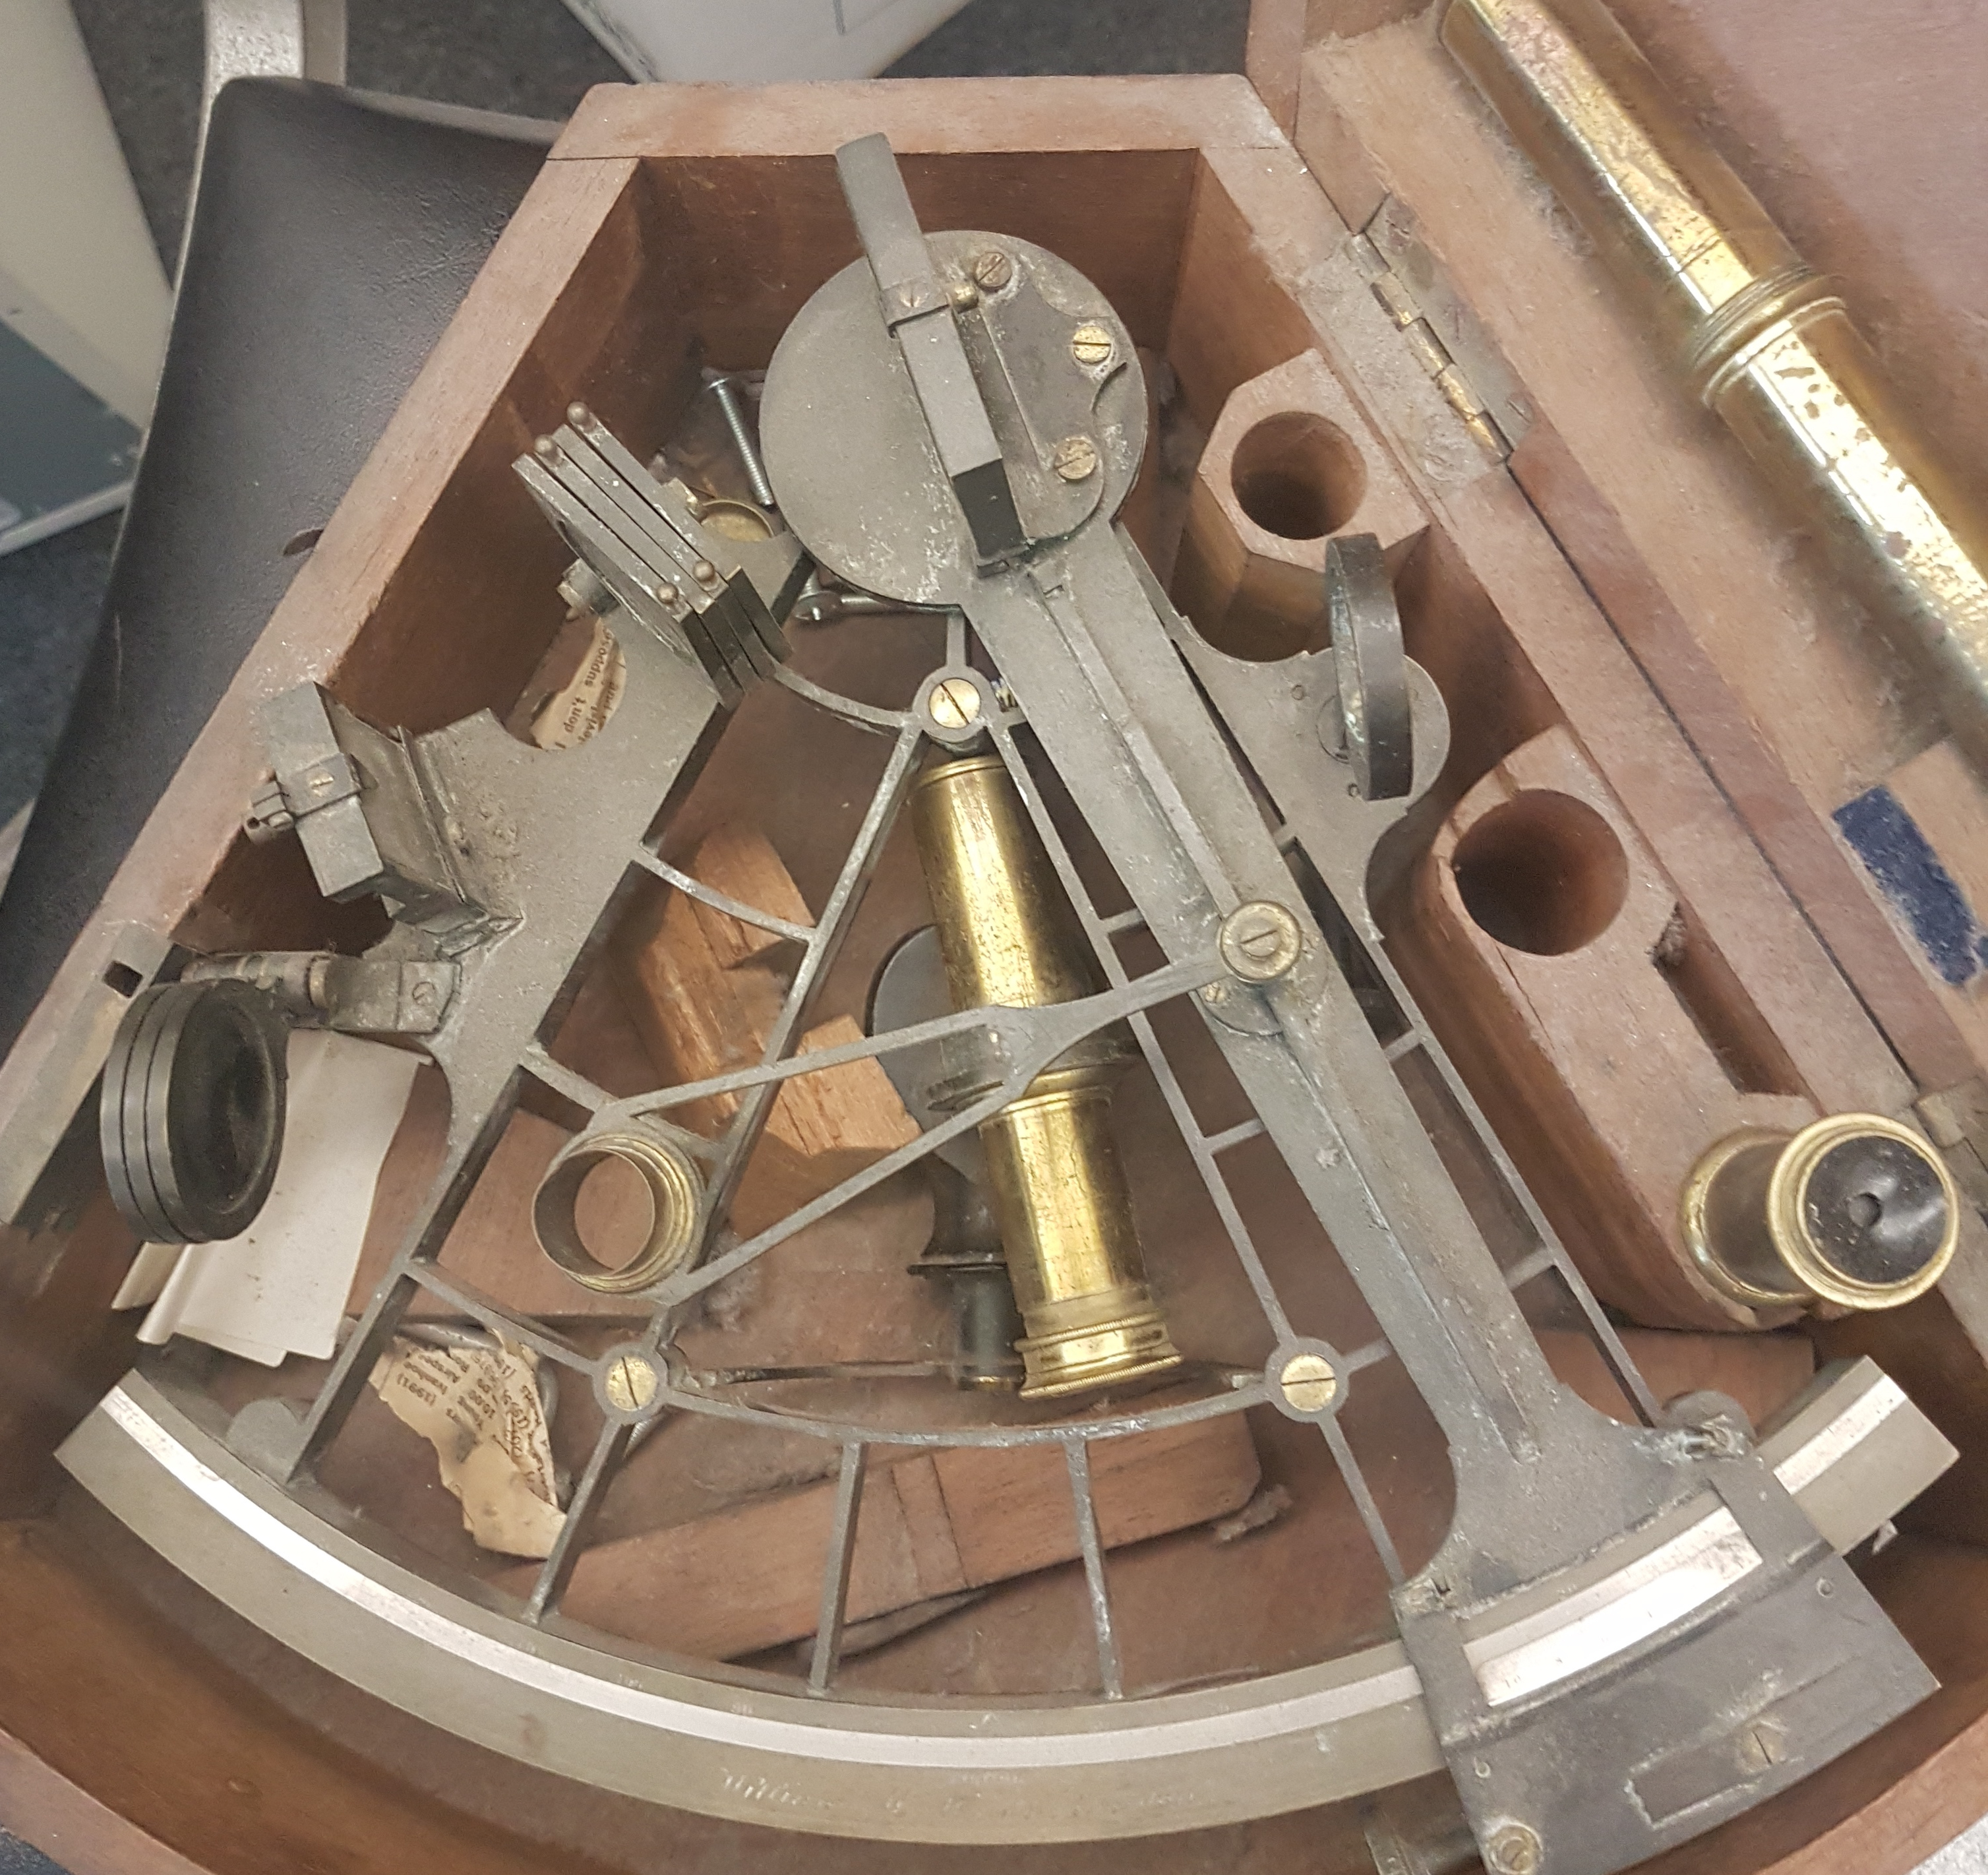
\includegraphics[scale=0.05]{McMillan1a}
\end{center}
}
\frame{ 
\frametitle{My Sextant}\small
My Tamaya is  a modern Japanese working sextant that I carry on my boat. It has worm gear worked by a  drum calibrated in minutes and a Vernier to read to 0.2 minutes of arc. It has a prismatic monocular telescope for viewing stars.

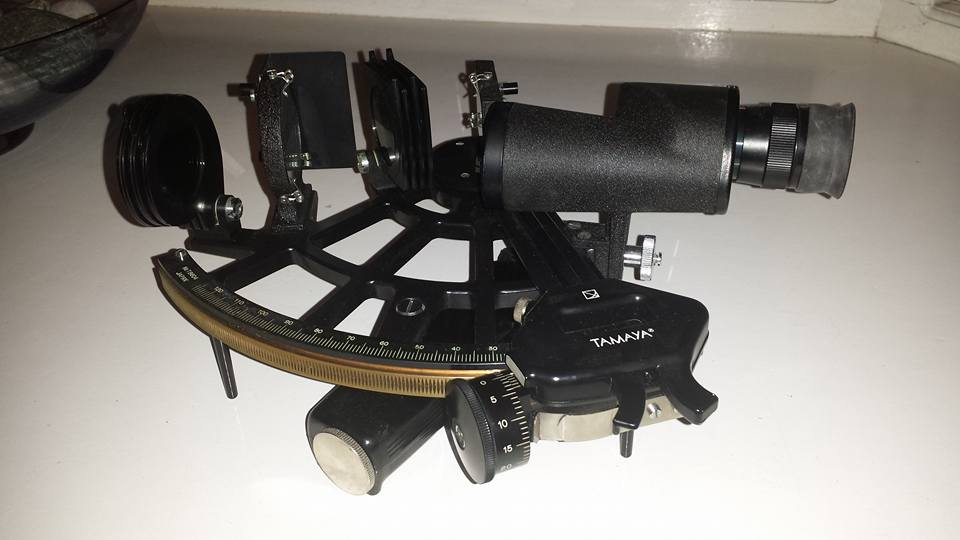
\includegraphics[scale=0.35]{Tamaya}
}
\end{document}